\documentclass{sigchi}

% Copyright
\CopyrightYear{2022}
% \setcopyright{acmcopyright}
% \setcopyright{acmlicensed}
\setcopyright{rightsretained}
% % DOI
% \doi{https://doi.org/10.1145/3313831.XXXXXXX}
% % ISBN
% \isbn{978-1-4503-6708-0/20/04}
% %Conference
% \conferenceinfo{UIST'20,}{October  20--23, 2020, Minneapolis, MN, USA}
% %Price
% \acmPrice{\$15.00}

\pagenumbering{arabic}

% Load basic packages
\usepackage{graphics}      % for EPS, load graphicx instead 
\usepackage[T1]{fontenc}   % for umlauts and other diaeresis
\usepackage{txfonts}
\usepackage{mathptmx}
\usepackage[pdflang={e\setlength {\marginparwidth }{2cm}n-US},pdftex]{hyperref}
\usepackage{color}
\usepackage{booktabs}
\usepackage{textcomp}
\usepackage{xcolor}
\usepackage{listings}
\usepackage{soul}
\usepackage{float}
\usepackage{amsmath}
\numberwithin{figure}{subsection}
\usepackage[font=small, bf,skip=5pt]{caption}
\captionsetup{belowskip=-10pt}
% \DeclareCaptionFont{white}{\color{white}}
% \DeclareCaptionFormat{listing}{%
%   \parbox{\textwidth}{\colorbox{gray}{\parbox{\textwidth}{#1#2#3}}\vskip-4pt}}
% \captionsetup[lstlisting]{format=listing,labelfont=white,textfont=white}
\lstset{numbers=left,xleftmargin=3em,frame=single,framexleftmargin=2.5em,escapeinside={(*@}{@*)},captionpos=b,xrightmargin=-\fboxsep, language=Python,firstnumber=1,
numberfirstline=true,belowskip=-2pt}
\lstset{basicstyle=\small\ttfamily, columns=fullflexible}

% Some optional stuff you might like/need.
\usepackage{microtype}        % Improved Tracking and Kerning
% \usepackage[all]{hypcap}    % Fixes bug in hyperref caption linking
\usepackage{ccicons}          % Cite your images correctly!
% \usepackage[utf8]{inputenc} % for a UTF8 editor only
\usepackage{xcolor}

\def\plaintitle{Design Study for a Geospatial-Video Data Analysis Query Language}
\def\plainauthor{
    Chanwut Kittivorawong,
    Shadaj Laddad,
    Andrew Lenz,
    Amy Lu
}
\def\plainkeywords{User Studies; Geospatial-Video Data; Data Model; Query Language}
\def\plaingeneralterms{Documentation, Standardization}

% llt: Define a global style for URLs, rather that the default one
\makeatletter
\def\url@leostyle{%
  \@ifundefined{selectfont}{
    \def\UrlFont{\sf}
  }{
    \def\UrlFont{\small\bf\ttfamily}
  }}
\makeatother
\urlstyle{leo}

% To make various LaTeX processors do the right thing with page size.
\def\pprw{8.5in}
\def\pprh{11in}
\special{papersize=\pprw,\pprh}
\setlength{\paperwidth}{\pprw}
\setlength{\paperheight}{\pprh}
\setlength{\pdfpagewidth}{\pprw}
\setlength{\pdfpageheight}{\pprh}

% Make sure hyperref comes last of your loaded packages, to give it a
% fighting chance of not being over-written, since its job is to
% redefine many LaTeX commands.
\definecolor{linkColor}{RGB}{6,125,233}
\hypersetup{%
  pdftitle={\plaintitle},
% Use \plainauthor for final version.
  pdfauthor={\plainauthor},
  pdfkeywords={\plainkeywords},
  pdfdisplaydoctitle=true, % For Accessibility
  bookmarksnumbered,
  pdfstartview={FitH},
  colorlinks,
  citecolor=black,
  filecolor=black,
  linkcolor=black,
  urlcolor=linkColor,
  breaklinks=true,
  hypertexnames=false
}

% create a shortcut to typeset table headings
% \newcommand\tabhead[1]{\small\textbf{#1}}

% End of preamble. Here it comes the document.
\setlength {\marginparwidth}{2cm}
\begin{document}

\title{\plaintitle}

\numberofauthors{4}
\author{%
  \alignauthor{Chanwut Kittivorawong\\
    \affaddr{UC Berkeley, USA}\\
    \email{chanwutk@berkeley.edu}}\\
  \alignauthor{Shadaj Laddad\\
    \affaddr{UC Berkeley, USA}\\
    \email{shadaj@berkeley.edu}}\\
  \alignauthor{Andrew Lenz\\
    \affaddr{UC Berkeley, USA}\\
    \email{andrew.lenz@berkeley.edu}}\\
  \alignauthor{Amy Lu\\
    \affaddr{UC Berkeley, USA}\\
    \email{amyxlu@berkeley.edu}}\\
}

\maketitle

\newcommand{\note}[2]{\textcolor{#1}{[#2]}}
% Hide Comments
% \newcommand{\note}[2]{}
\newcommand{\mick}[1]{\note{blue}{Mick: #1}}
\newcommand{\shadaj}[1]{\note{cyan}{Shadaj: #1}}
\newcommand{\andrew}[1]{\note{teal}{Andrew: #1}}
\newcommand{\amy}[1]{\note{orange}{Amy: #1}}
\newcommand{\todo}[1]{\note{red}{Todo: #1}}

% !TEX root =  ../geospatial-video.tex

\begin{abstract}
% Geospatial-Video data analysis tasks require storing and retrieving videos to answer questions about their data.
Geospatial-video databases help data scientists store their video data efficiently,
but many of them do not provide intuitive query languages for the data scientists to retrieve the data back.
Databases with intuitive query languages provide data abstractions that hide their internal data representations.
These data abstractions limit the number of operations that data scientists can perform on their data. In this paper, we address the failure for existing languages to easily enable queries to video frames, as identified through need-finding interviews with users of geospatial-video query languages. 
%As a response, we propose improvements to the expressiveness of the existing geospatial-video data analysis tool.
We focus on its data abstraction and query language design.
Our new data abstraction additionally includes a video frame data-type.
Our new query language provides operations for users to reason about video frames in their data.
\end{abstract}

% ACM Classification
% https://dl.acm.org/ccs/ccs_flat.cfm
\begin{CCSXML}
<ccs2012>
   <concept>
       <concept_id>10003120.10003121.10003122.10003334</concept_id>
       <concept_desc>Human-centered computing~User studies</concept_desc>
       <concept_significance>500</concept_significance>
       </concept>
   <concept>
       <concept_id>10002951.10002952.10003197</concept_id>
       <concept_desc>Information systems~Query languages</concept_desc>
       <concept_significance>500</concept_significance>
       </concept>
   <concept>
       <concept_id>10002951.10003227.10003236.10003237</concept_id>
       <concept_desc>Information systems~Geographic information systems</concept_desc>
       <concept_significance>300</concept_significance>
       </concept>
 </ccs2012>
\end{CCSXML}

\ccsdesc[500]{Human-centered computing~User studies}
\ccsdesc[500]{Information systems~Query languages}
\ccsdesc[300]{Information systems~Geographic information systems}

% Author Keywords
\keywords{\plainkeywords}

% Print the classification codes
\printccsdesc

% !TEX root =  ../geospatial-video.tex

\section{Introduction}

Capturing moments with video cameras is easy, and storage costs for storing video data is cheap. Video cameras have thus become a widely used tool to document moments through visual information.
However, visual information of video data is unstructured, making it difficult to store and look-up.
Processing and analyzing is often labor- and time-intensive for the data scientist. 
A common approach is to extract spatial and temporal information from the video data, using computer vision techniques~\cite{redmon:yolo,wojke:deepsort}.
The extracted information makes the data more structured and easier to organize.
We can them map the spatial information to the real-world location, becoming geospatial information.
Geospatial information helps data scientists to make sense of the video data as they correlate with the real world.
However, we still lack easy-to-use and expressive language to retrieve and explore the data.

Our goal for this project is to design a language that makes it easier for data scientists to search and explore massive geospatial-video datasets. We explore two geospatial-video data analysis use cases, and use them to shape the design of our tool:

\begin{itemize}
    \item
    \textbf{Autonomous Driving}: Scenic~\cite{fremont:scenic} is a language for generating visual scenes, specifically for autonomous vehicle training data.
    %An researcher working on creating autonomous driving technologies usingon validating visual scenes generated~\cite{kim:scenic-validation},
    by comparing the scenes with a real-world autonomous vehicle video data~\cite{ceasar:nuscenes}.
    A Ph.D. student in Computer Science is working on validating visual scenes generated~\cite{kim:scenic-validation},
    by comparing the scenes with a real-world autonomous vehicle video data~\cite{ceasar:nuscenes}.
    
    \item
    \textbf{Evident of Misconduct:}
    Data journalists often have large banks of video data, but not nearly enough time to look through these data. This may hinder the ability to accurate retrieve evidence involved in things like police misconducts or false court statements.
\end{itemize}

In order to uncover what are the essential user necessities of a geospatial-video analysis tool, introduce new features to expediate workflows, and decrease barrier-to-entry for working on these important problems, we conduct user interviews related to the two use cases above.

% \andrew{Why hasn’t this topic been studied before, or why haven’t prior studies answered the questions you’re answering?
% One issue with developing this tool is that in order to use it,
% there must be an annotated dataset that contains information such as the geographical location of objects and labels of the elements in the video.
% However, some of these concerns could be amended by using a computer vision model to label the video,
% so we will not address that in this paper.}
We have explored prior attempts on geospatial-video data analysis tools.
VisualWorldDB~\cite{haynes:visualworlddb} presents a new data model to help users make sense of their video data after they are stored in the database.
However, the work focuses heavily on the data storage system and optimizations.
The proposed SQL-like query language is difficult to use as it exposes its internal data tables from which users can query.
Apperception~\cite{ge:apperception} is built on top of the VisualWorldDB idea and aims to improve its usability.
Apperception has a much simpler query language compared to VisualWorldDB.
In the attempt, Apperception hides all the the internal data table and present a new data abstraction to users.
As a result, the query language cannot express some data exploration questions.
CLIP~\cite{radford:clip} is a large language model capable of generating video frames from a natural language description as the prompt. 
However, the results are not deterministic, and it is difficult to query geospatial or temporal information.

In this project we made following contributions:
\begin{enumerate}
    \item
    We interviewed a data journalist and a computer science undergraduate,
    who are working on geospatial-video data analysis tasks.
    \item
    We designed a Python~\cite{van:python} programming tool based on prior works and participants' need from the interviews.
    Our tool presents an easy-to-understand data abstraction that will allow programmers of any experience level to easily explore large geospatial-video databases. Our tool also provide an expressive domain-specific language for users to explore their geospatial-video datasets through the data abstraction we provided.
    \item
    Our tool is designed to be extensible.
    Users will be able to extend our language with their custom functions.
    These custom functions help the users to express the queries that our provided query language cannot.
    \item
    We design a Graphical User Interface (GUI) for non-programmer to apply the same principle that our python tool provides but without programming experience.
\end{enumerate}

% !TEX root =  ../geospatial-video.tex

\section{Related Work}

\subsection{VisualWorldDb}
In this paper~\cite{haynes:visualworlddb}, the author introduces the concept of Visual World Applications (VWAs).
VWAs are applications that rely on spatial and temporal information from visual data.
The authors present VisualWorldDB: a video database management system optimized for VWAs.
With VisualWorldDB, users can create a \emph{world} that represents the real world.
Then, users can ingest multiple geospatial-videos into the \emph{world}.
VisualWorldDB then places all the \emph{visual objects} present in the videos into the \emph{world}.
Each \emph{visual object} has properties that include its location in the real world.
After the users have all the \emph{visual objects} added to the \emph{world},
they can query for these \emph{visual objects} instead of their videos.
In the end VisualWorldDB retrieves the videos associated with the \emph{visual objects} queried.

Despite the simplified data model, VisualWorldDB focuses on its storage systems and optimization.
The paper does not go into much discussion about VisualWorldDB's query language.
The paper presents an example program in VisualWorldDB's language to ingest videos into a \emph{world}.
The language has a SQL-like syntax that expose internal data tables for users to manually input rows of data themselves.
However, this approach is not intuitive to users.
First, the programs that users write are prone to errors.
All the internal data tables should have an invariant that keep the \emph{world} representation valid.
However, users have access directly to the internal data table,
so they can unintentionally break some of the invariant.
Second, the program that the user writes is verbose.
To add a video camera into a created \emph{world}, users need to:

\begin{enumerate}
    \item
    Add the camera as an object to the world into an Objects table.
    \item
    Add the position of the camera as a point in to the world into a Point table.
    \item
    Add the orientation of the camera as another point into the world into the same Point table.
    \item
    Add a video file associated with the camera into the created world.
\end{enumerate}
Adding a camera to the \emph{world} could be done as one operation --
instead, we need four operations to perform this task. In this project, we take inspiration from this \emph{visual world} concept.

\subsection{Apperception}
Apperception~\cite{ge:apperception} has a similar \emph{world} concept as VisualWorldDB but with a more usable Application Programming Interface (API).
Apperception stores all the geospatial data in MobilityDB~\cite{zimanyi:mobility}. However, it provides a Python API for users to interact with its geospatial-video data storage.
Apperception also provides a Python \emph{World} object that represent a \emph{world}.
There are multiple operations that users can do with a \emph{world}.
\begin{itemize}
    \item
    \textbf{\texttt{add\_camera}} to add a camera and video to the \emph{world}.
    Compared to VisualWorldDB, users only need one operation to add a camera to a \emph{world}.
    \item
    \textbf{\texttt{recognize}} to extract objects from an existing video and place them into the \emph{world}.
    \item
    \textbf{\texttt{filter}} to filter only objects that the user is interested in.
\end{itemize}
After all the operations done, users will have a \emph{World} that contains only the objects that they are interested in.
Then, they can use a \textbf{\texttt{get\_*}} method to observer the state of the world.
\begin{itemize}
    \item
    \textbf{\texttt{get\_trajectory}} gives users the trajectory of each of the objects in the world.
    The users can then use an \textbf{\texttt{overlay\_trajectory}} method to overlay the trajectories into the original video.
    \item
    \textbf{\texttt{get\_videos}} gives the videos of all the objects in the world.
\end{itemize}

Apperception's interface is easy to use and not verbose.
It wraps around the internal geospatial-video data storage,
so the users do not have direct access to the data table.
As a result, it is less likely for them to accidentally violate the data store invariant.

A \emph{World} is immutable, which means that it cannot be modified.
Any operation done to a \emph{World} create a new \emph{World} that represents the original one with the operation applied to.
This approach for making a \emph{World} immutable helps users to easily reason about the program they have written.
In addition, having a immutable DataFrame-style syntax is common in tools~\cite{mckinney:pandas, pandas, wickham:dplyr} for data exploration tasks.
Users who are already familiar with data exploration tools could learn how to use Apperception quickly.

However, Apperception's language is designed for users to find objects in a \emph{World}.
It is difficult for users to describe a query that can find a specific moment of an object using only Apperception language.
For example, if a user has an hour-long video that capture the same car for the whole video.
The car crashes at 45th minute of the video.
The user can use Apperception language to query for a car that crashes.
Apperception will return a \emph{World} that only contains the car.
But, Apperception cannot provide the information about the when the incident occurs.

Our project will build on top of Apperception's language: we aim to address the problems with Apperception language, specifically, that it is not expressive enough to describe complex data exploration questions.

\subsection{Rekall}
Rekall~\cite{fu:rekall} is another video data analysis tool that we looked into.
Rekall presents an abstraction for video data for its video frames.
Rekall does not organize videos as a \emph{world} --
instead it simply organize them as collections of video frames.
Rekall also provide a \textbf{\texttt{filter}} method like in Apperception, 
but instead of filtering by objects, Rekall's \textbf{\texttt{filter}} filters only the frames that the user is interested in.

This abstraction and operator is helpful to our project because it fills in the main disadvantage of Apperception.
Our project will be integrating the by-frame abstraction to our data model and query language.

% \mick{todo: CLIP/LiveReel?}
% \todo{What alternative techniques have people used to work on this problem?}
% \todo{What techniques did you adopt from others?}

\subsection{Fructure for Racket}
When considering the design for our user interface, we were inspired by Andrew Blinn's Fructure for Racket~\cite{blinn:fructure}, a projectional editor that allows users to either type code or select code via mouse to fill in holes in a program.
Projectional editors are efficient for basic code-editing activities \cite{berger:projection} and useful for educational uses, particularly as they prevent syntax errors \cite{santos:javardise, weintrop:block-based}, which is important for our users who are less experiences with coding.
On the other hand, our more experienced programmers may want to type code the traditional way: Fructure's flexibility allows users to type in the holes rather than just scrolling through the list, and we would implement this as well.


% !TEX root =  ../geospatial-video.tex

\section{Interviews}

\todo{What research questions drove the design of the study?}
In our user interviews, we 

\todo{How did you collect data about your target population?}

\todo{How did you find participants?}

\todo{How did you select participants?}

\todo{What procedure did you use for collecting data?}

\todo{What materials, if any, did you show participants?}

\todo{What data did you collect?}




\todo{What did you learn from the user data?}

\todo{How did you learn it?  What led you to these conclusions?  Be specific.}

\todo{What quotes, stories, numbers, or patterns back up these conclusions or offer extra detail?}

\todo{Which conclusions surprised you?}

\todo{How did your conclusions from the user data affect what you did next?}

\todo{How should your conclusions from the user data affect what future researchers do?}

\todo{andrew?}


In order to identify short-comings for current tools and guide the design of our work, we conducted contextual inquiry and observed users performing tasks involving geospatial video analysis using existing tools. An area of the pipeline which we were especially interested in is how researchers specify queries that identify situations with multiple objects, potentially with some specific behavior over time. The following section discusses the findings from our two interviews in greater detail.

% Who are your formative study participants?
% Lisa Pickoff-White: KQED
% Investigating videos for police misconduct cases
% Yousef Helal: Undergraduate students at Berkeley
% Working on translating query from Scenic to Apperception query
% What protocol are you using during sessions with participants?
% Lisa
% Contextual Inquiry
% Yousef
% Contextual Inquiry
% Structured questions asking participant to rank choices
% Explanation: With multiple tasks, we will give him 2 queries for each task written with the old Apperception API and our new API. Then, we find Yousef's preferences for each task.
% What activities are your participants completing?
% Lisa
% We asked her to prepare a video investigating task.
% We also asked her to choose the task that takes about 20-30 minutes.
% Then, we will observe her workflow for the task.
% We might raise questions if we need any clarification.
% Yousef
% We asked him to prepare a query from Scenic to translate into an Apperception query.
% We can have 1-2 queries and would take around 5-10 minutes.
% We also will ask him to bring a Scenic query that is difficult to write in Apperception.
% Show him our new design and how it works.
% Give multiple queries in our new design
% Ask him to give a short description of each of the queries.
% What data are you collecting?
% Lisa
% Screen recording (need their permission)
% Workflow for her video data exploration. Which parts are slow?
% Yousef
% Screen recording (need their permission)
% The query that he decides to write in Apperception.
% What are the questions that Apperception cannot describe?
% Comparing the API from Apperception and ours
% The confidence level that they will be able to answer their question with our new API.
% How are you going to analyze that data?
% Record their pain points during the interviews. Afterward, we try to group them into larger concepts
% Take general notes on parts of the analysis process that cause the study participants to pause, as these may be aspects of the query creation process that we can optimize
% For Yousef, the API examples we provide will be categorized ahead of time into the types of constructs (functional, declarative, etc.) that they use; we will then attempt to identify how these constructs affected the confidence scores




\subsection{Data Journalist}
User L is a data journalist at a public radio station who must look at video evidence on the order of thousandsto collect and report on evidence, specifically surrounding police misconduct. With permission, we recorded L performing the video queries required for this task. In L's workflow, she goes through several videos and makes quick notes on their utility for her aim; for relevant videos, she ``clicks around a little" through frames to roughly orient herself with what is happening in the scene. Once key frames are identified, L takes 



\todo{focus on why we need to filter by frame instead of just filtering by objects like in apperception}
\todo{to scope down the part of each video that are as of useful to them}

\subsection{Programmer}
\todo{focus on our syntax and data model that it is understandable}
\todo{focus on the part where he suggests us to implement a syntax where users can filter by frame and then switch to filter by objects}
% !TEX root =  ../geospatial-video.tex

\section{Dataset}
%\todo{to focus: \\
%- explain briefly about the dataset, what for, shape of the data.
%- how we transform the dataset to fit our data model.
%}

For our prototype, we use the nuScenes dataset~\cite{ceasar:nuscenes}, a collection of camera, lidar, and radar images to facilitate autonomous driving research. Data is collected from 15 hours of driving data in Boston and Singapore, and key frames are sampled at a rate of 2Hz for labeling by human annotators, resulting in a rich collection of information suitable for various downstream needs in autonomous driving research. The structure of the decomposition of video frames into data and annotation structure was a good representative of geospatial settings for our language design.


% !TEX root =  ../geospatial-video.tex

\section{Data Model}
\label{section:data-model}

To interface with the data, the user uses the \textit{Annotation}, \textit{Instance}, \textit{Frame}, and \textit{Video} abstractions.
\begin{itemize}
    \item 
    \textbf{\textit{Video}} represents a video file.
    \item 
    \textbf{\textit{Frame}} represents a video frame in a video file.
    \item 
    \textbf{\textit{Instance}} represents an object that presents in a video. An \emph{Instance} can be present on a video spanning over multiple frames as shown in Figure~\ref{fig:abstraction}.
    \item 
    \textbf{\textit{Annotation}} represents properties of an \emph{Instance} for a specific \emph{Frame}.
\end{itemize}
Figure \ref{fig:abstraction} illustrates this data model in greater detail.
Each video is denoted by an unique scene ID, and frames are indexed by the order in which they appear.
All instances have an unique instance token which can be used to query specific properties for that instance specifically.
By passing the scene ID, the user can load the video with corresponding annotations and properties needed for downstream tasks.
The user may also directly instantiate any Frame and Instance directly from the nuScenes database, if provided with the frame order and instance token in addition to the scene ID.
All metadata are stored in Annotations, with the exception of ``Category" (e.g. ``car", ``person"), which is an attribute in \textit{Instance}.

\newcommand{\dataModelCaption}{
The wealth of image, annotation, spatial, and temporal information in geospatial data is simplified into in our language into Video, Frame, Instance, and Annotation.
A video consists of several consecutive frame, which point to a specific image, and instances (e.g., cars, pedestrians) may persist through many frames.
Each instance contains a category attribute, and an annotations attribute for accessing more detailed metadata of interest.
}

\begin{figure*}[ht]
    \centering
    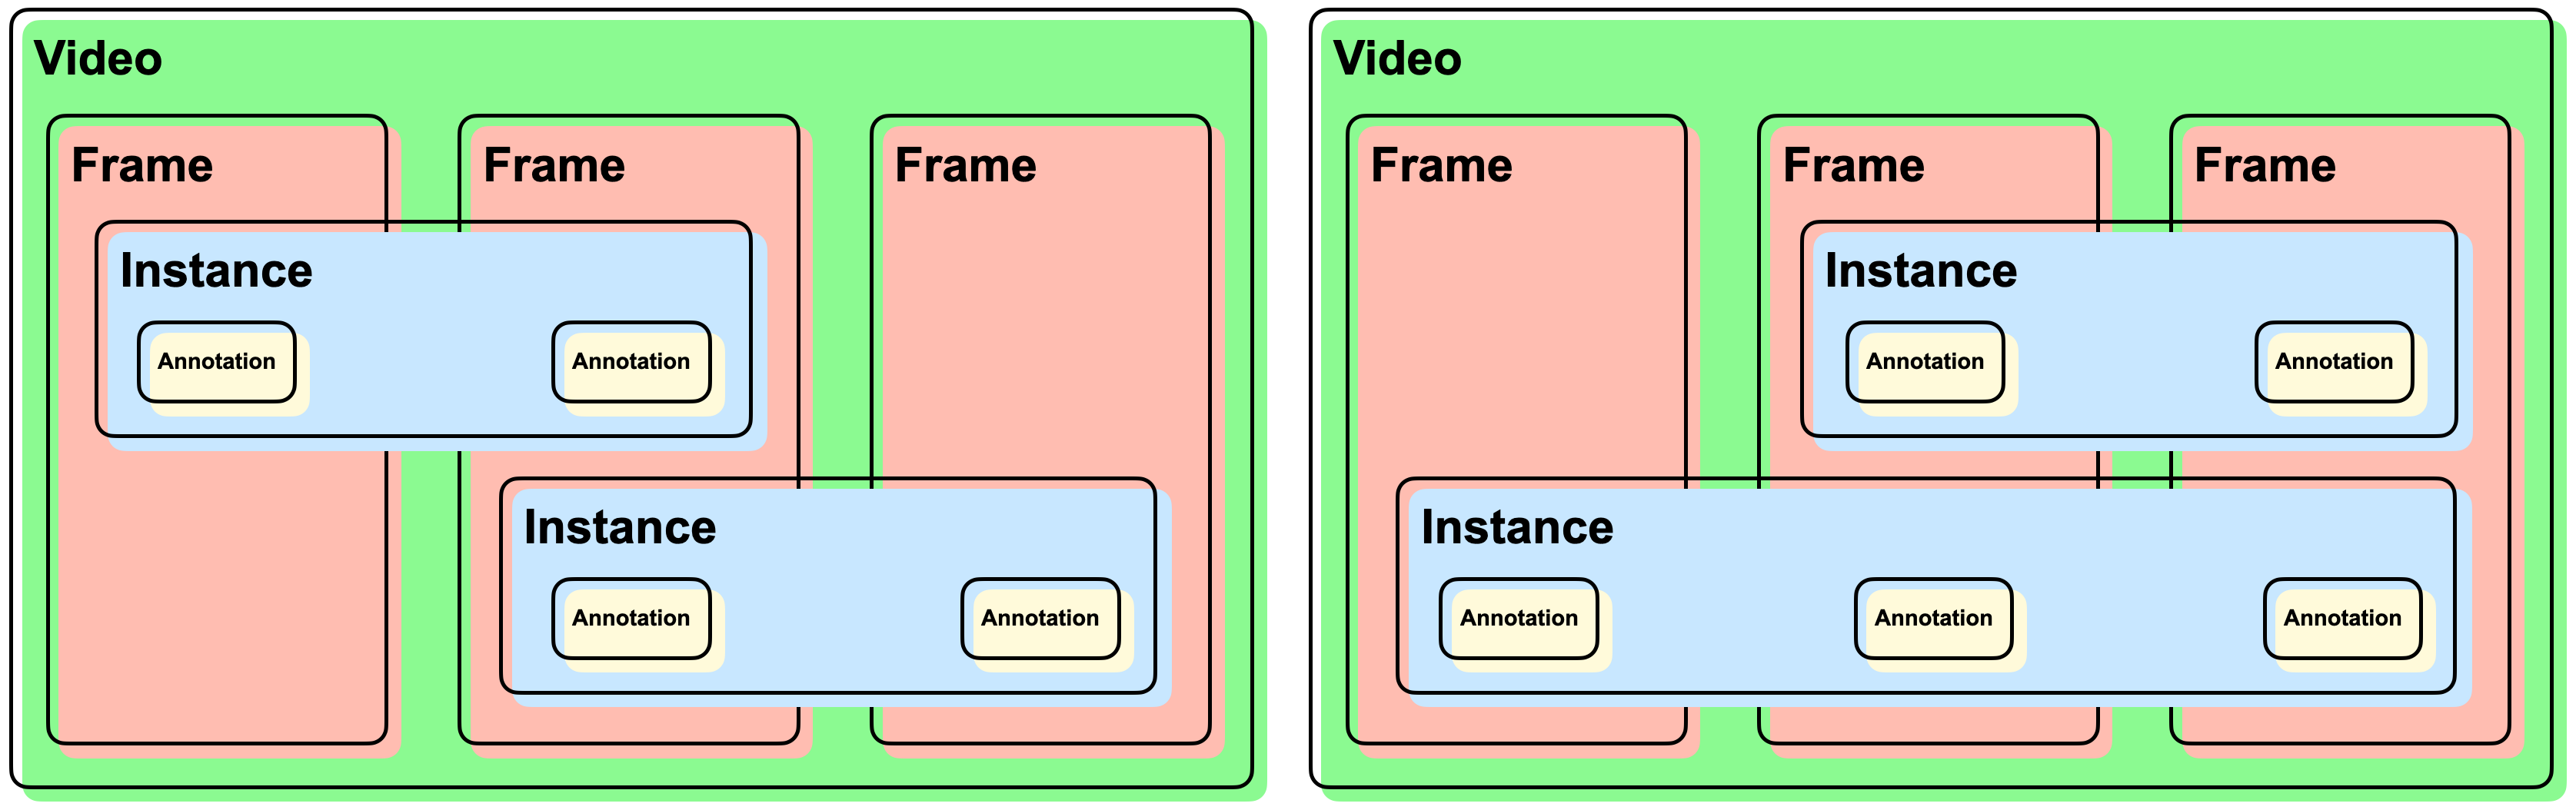
\includegraphics[width=\textwidth]{figures/data-abstraction.png}
    \caption{\dataModelCaption}
    \label{fig:abstraction}
\end{figure*}

\newcommand{\dataHierarchyCaption}{
The hierarchy of our data type.
Users can start exploring they geospatial-video data from \emph{Videos}.
Then, they can choose to explore the data through either \emph{Frames} or \emph{Instances}.
And from both \emph{Frames} and \emph{Instances}, they can explore further to \emph{Annotations}.
In addition, the users have the flexibility in switching between exploring \emph{Frames} and \emph{Instances}.
}

\begin{figure}[ht]
    \centering
    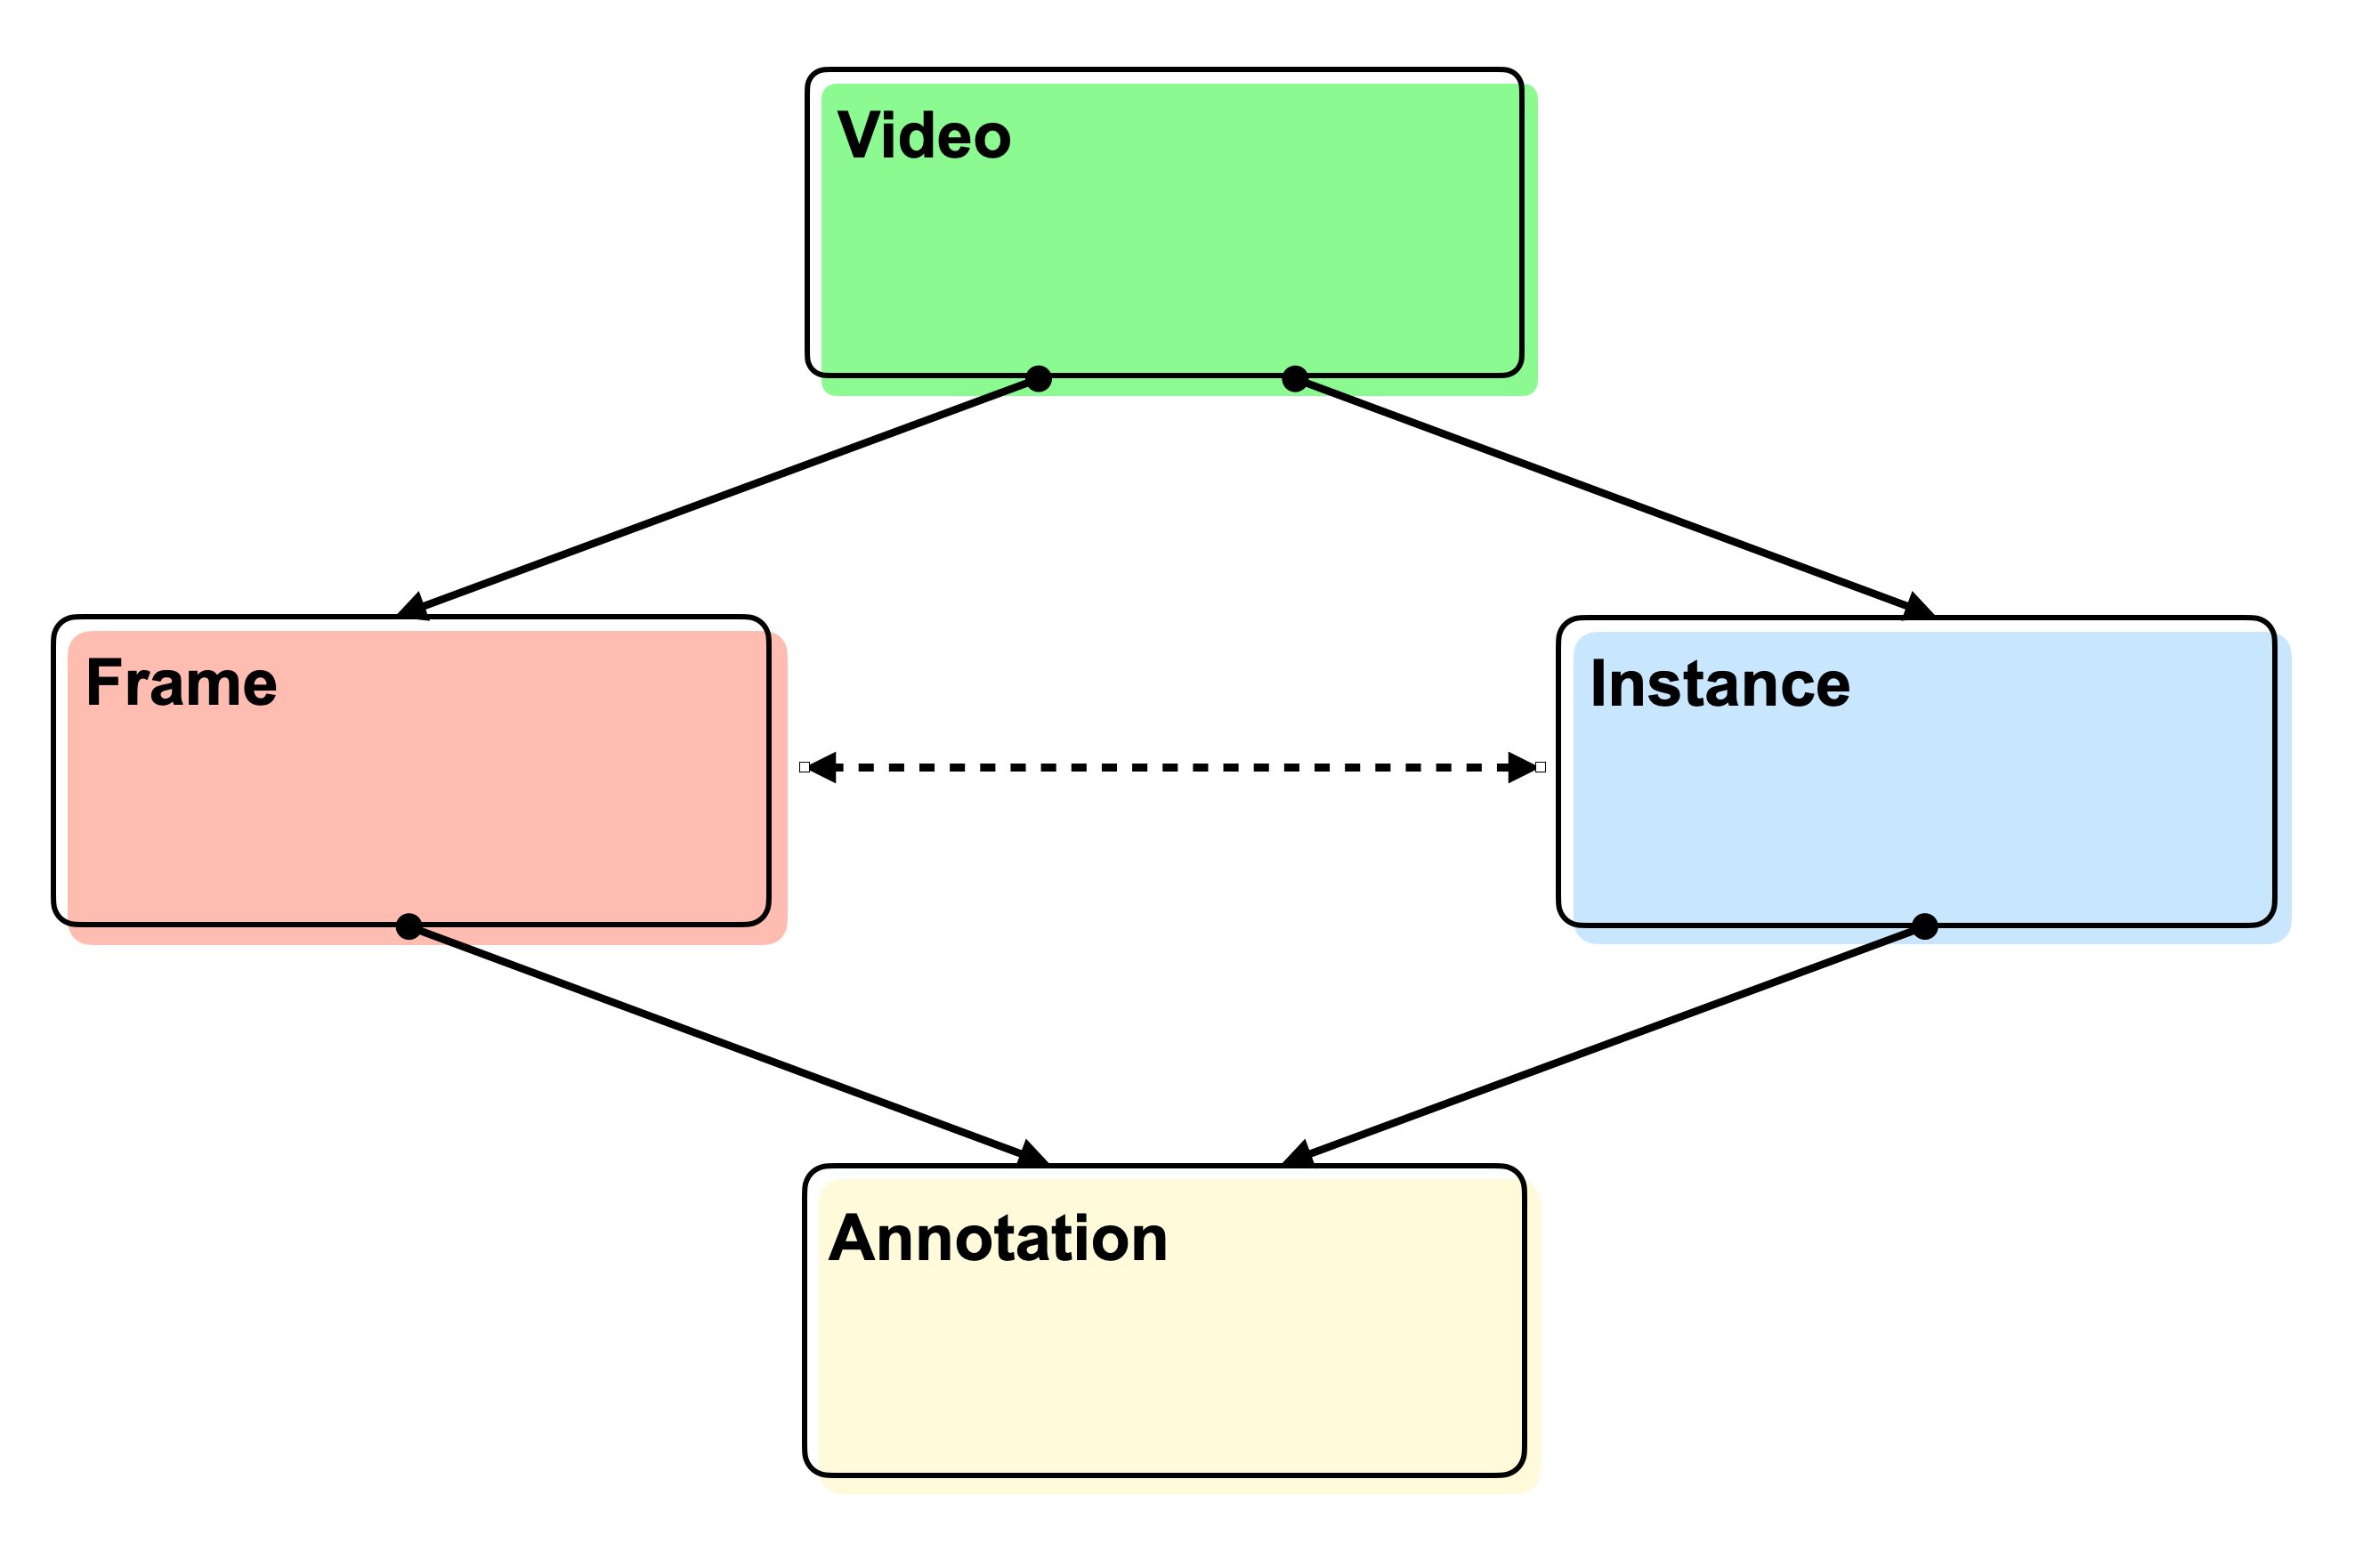
\includegraphics[width=\columnwidth]{figures/data-hierarchy.png}
    \caption{\dataHierarchyCaption}
    \label{fig:hierarchy}
\end{figure}

Our data model is an improvement to Apperception's data model.
In Apperception, users mostly interact with \emph{World}, \emph{Video}, and \emph{Instance}, and do not have access to individual frames of the video.
The output from Apperception can also only represent \emph{World} and \emph{Instance}.
In the new data model, users can interact with all of the data types shown in Figure~\ref{fig:hierarchy}.
This abstraction allows users to construct queries to answer more complex data exploration questions,
while not exposing the internal geospatial data store.

% !TEX root =  ../geospatial-video.tex

\section{Domain-Specific Language}
\begin{figure*}[t]
    \centering
    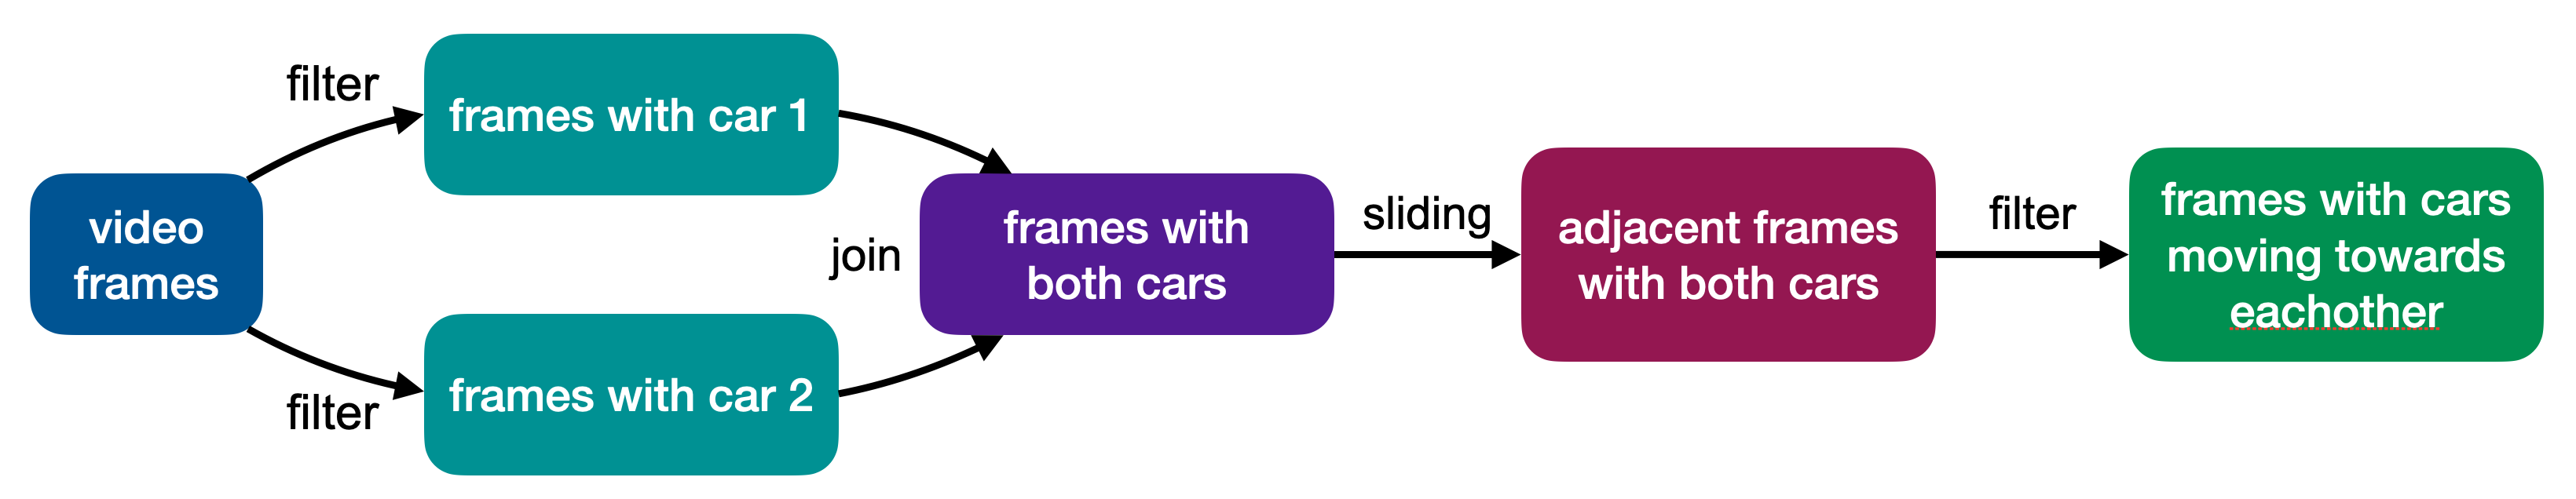
\includegraphics[width=\textwidth]{figures/declarative-dataflow.png}
    \caption{An example of a dataflow users can construct for a query that searches for adjacent frames where two specific cars are moving towards each other.}
    \label{fig:declarative_dataflow}
\end{figure*}

To address the pain points we noticed in our user interviews, we chose to design a new language for describing queries over geospatial video data as a domain-specific language embedded in Python. Instead of building a new language from scratch, which would require designing a new syntax and editor integrations that users would have to learn about, we are able to inherit the large ecosystem of existing tooling around Python. Furthermore, some potential users of our system (such as User Y) are already familiar with Python, which makes it easier to adopt our language.

\subsection{Design Guidelines}
There are three key factors constraining the design of our language: incremental query creation, support for using the language through a graphical user interface, and supporting queries that combine predicates over time and space. Before we dive into how we design the language around these constraints, let us walk through how we derived the factors based on our user-studies and their consequences on the space of language designs.

\subsubsection{Incremental Queries}
Across the interviews, a key pattern that stuck out was the process by which the participants would identify portions of video that were of interest---either by manual scrubbing through video files or the creation of queries in existing systems. Rather than define the end-to-end query, the participants would start with a coarse grained search, looking for portions of the video that are likely to have the information they are looking for. Across these sections, the participants would then refine their search/query by playing back the video in real-time or querying individual frames in more detail.

Our insight from this observation was that users of video query languages will want to develop the query incrementally, where they start with a query that identifies sections of the video with general patterns related to their specific goal--such as the presence of multiple cars in the same frame--and iteratively refine it to identify the specific scenario--such as cars moving towards each other--while receiving feedback from the query engine.

Supporting incremental query creation places significant constraints on the design of the language since the language must offer modular APIs to support users adjusting their query pipelines over time and must also have a performant runtime that can execute updated queries efficiently. Furthermore, it requires us to ascribe meaning to intermediate steps of a query, including complex concepts such as windows over time or groups of objects, so that users can see the results of each component of their pipeline.

\subsubsection{Graphical User Interface}
Based on our interview with User L, who works on data journalism but primarily uses manual scrubbing methods to query videos rather than writing code, we identified that a key feature to make our language useful is offering a graphical interface for constructing programs for users who are not comfortable with text languages. At the same time, however, we want to support a lower-level Python API for constructing queries that expert users such as User Y would be more comfortable using.

To support this graphical interface, we decided to implement a layer on top of the Python API with mappings from each concept in Python to features in the interface. This architecture means that the low-level API should be strongly typed, since types in the API are important to constrain the programs in the graphical interface to those that are executable by construction. Furthermore, it requires us to include several built-in APIs for common scenarios to reduce the overhead of describing various queries.

\subsubsection{Queries over Time and Space}
Finally, we observed in both interviews that queries over video data often require repeatedly moving between the axis of time and detected objects, something that existing query systems do not support. For a concrete example, consider an query over autonomous vehicle data that is looking for collisions. We want to find chunks of the video where two cars are moving to each other, but this requires predicates that both reason about multiple frames together and multiple objects together. After a user writes a query to identify cars, they will need to identify \emph{frames} with multiple cares, and then process windows of frames to check if the detected objects are moving towards each other.

As we noticed in our interview with User Y, queries like this are difficult or impossible to describe with existing query languages, which either focus exclusively on time or objects as the primary axis being queried over. We aim to address this in our design by providing APIs that mix these two concepts together, enabling queries such as filtering over the properties of objects in windows of time. This requires us to extend the data model, as we discussed in the previous section, and also provide APIs for switching between the frame and instance views of video data.

\subsection{Language Design}
With these design goals, we decided to develop a DSL based on declarative and functional programming principles. Rather than writing out queries as imperative statements that mutate data, have unclear dependencies, and use hard-to-optimize control constructs, this approach allows us to optimize and execute the queries users write from a global perspective. By modeling queries as dataflows, such as the example in Figure~\ref{fig:declarative_dataflow}, our language can also provide high-quality intermediate feedback since every intermediate node can be mapped to output samples. Finally, the declarative approach makes it simpler to build a graphical interface, since the dataflow model corresponds to a natural visual model of connecting primitive operations with dependencies.

Our DSL consists of four core types corresponding to the elements of our data model: videos, frames, instances, and annotations. To develop dataflows over these structures, we then provide collection types wrapping these elements, which represent nodes that will process incoming streams of video data. In the time domain, we also include a collection type that captures groups of frames rather than just individual elements, which is useful when performing tasks like tracking the motion of an object over a window of time.

To create complex queries, users can develop a dataflow pipeline by repeatedly transforming these collection types using functional operations. In addition to the classic transformations such as map, which transforms individual elements independent of each other, and filter, which applies a predicate to each element, we also include several operations specific to the domain of video data.

First, we include the \texttt{join} operator, which allows a user to combine multiple collections by matching elements with a specific property. This emits a collection containing groups of the elements in the original collections, and can be thought of as performing a crossproduct with a predicate. Rather than allowing an arbitrary condition, which can be difficult to evaluate efficiently, we constrain users to joining elements on properties which have already been computed. For example, users may join on frames, which will gather pairs of elements from both inputs that are present in the same frame.

Next, we add the \texttt{sliding(n)} transformation, which makes it possible to develop queries that reason about windows of time in the video rather than just individual points in time. 
When applied to a collection of frames, this operator produces a new collection containing groups of \texttt{n} adjacent frames. 
When applied to a collection of instances, however, this operation produces a collection of groups of \emph{annotations} corresponding to the states of the objects in adjacent frames.

Finally, we add APIs on collections of videos to flatten all frames (\texttt{flatten\_frames}) or instances (\texttt{flatten\_instances}) into a single collection. Users often have multiple video sources corresponding to a single event, so it is helpful to process all frames with a single query pipeline. Furthermore, we plan to support users specifying groups of instances that correspond across videos so that many sources can be combined into a global view of the scene, in a similar manner to the world view abstraction in Apperception.

Together, these constructs make it possible to express a wide variety of queries that process videos with both the frame-by-frame and per-instance views. By composing our video-specific APIs with the general functional APIs that support nested logic over frames or instances, users can easily build out the queries they need while ensuring that the pipeline is sufficiently modular to be adjusted in the future.

In our prototype implementation, we have implemented simple implementations of these APIs that iteratively process the input video streams in single-threaded Python logic. In future work, however, we plan to utilize the declarative nature of our DSL design to compile user-defined pipelines to efficient, parallel implementations.

% !TEX root =  ../geospatial-video.tex

\section{Extensions}

While we expect that the language will be sufficiently expressive to construct most types of queries, we also recognize that some of our users may not have the time, desire, or programming expertise to implement the functions that they may want to use to filter the videos. 
Therefore, we built out some of the possible helper functions that could be useful for filtering. We focused on exploring utility functions for the autonomous driving application, which already has a common set of query tasks we could take inspiration from.

These functions expect to be called within filter and thus all return boolean values. 
The ones provided below should take in the result of the sliding operation, as they intend to compare information about the instance across adjacent frames in order to determine something about the instance's movement.
However, these utility functions do not cover all possible use cases -- our language is designed such that a user can add their own utility functions as needed.

Utility functions for filtering: \\
(Note: \texttt{iX} and \texttt{fY} (where \texttt{X} and \texttt{Y} are whole numbers) will refer to Instances and Frames, respectively.)
\begin{itemize}
    \item \texttt{move\_away(i1, i2, f1, f2)}: \\
    This function calculates the distance between Instance \texttt{i1} and Instance \texttt{i2} in Frame \texttt{f1} and Frame \texttt{f2}, then compares these distances. 
    If the distance between the instances in Frame \texttt{f2} is greater than the difference between the instances in Frame \texttt{f2}, then we consider the instances to be moving away from one another.
    
    \item \texttt{accelerating(i, f1, f2, f3)}:\\
    This function uses the location of Instance \texttt{i} to determine if it has accelerated between Frame \texttt{f1} and Frame \texttt{f2}, and Frame \texttt{f2} and Frame \texttt{f3}. To determine this, it compares the difference in location between both pairs of frames: 
    if the difference between the locations in Frame \texttt{f2} and Frame \texttt{f3} is greater than the difference between the locations in Frame \texttt{f1} and Frame \texttt{f2}, we consider Instance \texttt{i} to have accelerated.

    \item \texttt{decelerating(i, f1, f2, f3)}: \\
    This function uses the location of Instance \texttt{i} to determine if it has decelerated between Frame \texttt{f1} and Frame \texttt{f2}, and Frame \texttt{f2} and Frame \texttt{f3}. 
    To determine this, it compares the difference in location between both pairs of frames: 
    if the difference between the locations in Frame \texttt{f2} and Frame \texttt{f3} is less than the difference between the locations in Frame \texttt{f1} and Frame \texttt{f2}, we consider Instance \texttt{i} to have decelerated.
    
    \item \texttt{stopped(i, f1, f2, tol: float)}: \\
    This function uses the location of Instance \texttt{i} to determine if it has stopped from Frame \texttt{f1} to Frame \texttt{f2}. 
    To determine this, it compares the difference in location between the two frames to the tolerance \texttt{tol}: 
    if the difference is greater than \texttt{tol}, we consider the instance to have moved; otherwise, it has stopped.
    
\end{itemize}
% !TEX root =  ../geospatial-video.tex

\section{User Interface}
Although we did not implement a user interface for the language, we were able to prototype some designs for such an interface. Based on these explorations, we propose a block-based projectional editor interface to provide the most convenience and accessibility for programmers, particularly those with less experience who we expect to use this tool. To facilitate this, we would allow users to fill the holes in skeleton queries by selecting entries from a drop-down menu which would also have a search bar; this will provide suggestions to users who want to explore the dataset, but also allow users who know what want to see to search for what they are looking for.  

As the output of a query in this language would be a series of clips or videos taken from the overall collection of videos,
we envision the interface as having a region in which the output of the queries are displayed.
However, this creates some problems when we have too many output videos.
To amend this, we would split the list of videos into multiple pages to prevent the tool from loading all the videos at once.
Then, we show the number of output videos.
If the number of output videos is too large, we suggest that the users add more filters to the output to narrow down their search.

\subsection{Mapping the Language to the Interface}

First, the tool will store the collection of videos as some variable,
which we will refer to as \texttt{videos}.
A typical query in our language is shown in the Listing \ref{fig:Map1}.

\begin{figure}[H]
    \fbox{\parbox{\linewidth}{\texttt{1\hphantom{ab}people = videos \textbackslash}\\
    \texttt{2\hphantom{abcdef}.flatten\_instances() \textbackslash}\\
    \texttt{3\hphantom{abcdef}.\textbf{filter}(\textbf{lambda} i: \textbackslash}\\
    \texttt{4\hphantom{abcdefghij}i.\textbf{property}["type"] == "person")}\\
    \texttt{5}\\
    \texttt{6\hphantom{ab}cars = videos \textbackslash}\\
    \texttt{7\hphantom{abcdef}.\textbf{flatten\_instances}() \textbackslash}\\
    \texttt{8\hphantom{abcdef}.\textbf{filter}(\textbf{lambda} i: \textbackslash}\\
    \texttt{9\hphantom{abcdefghij}i.\textbf{property}["type"] == "car")}\\
    \texttt{10}\\
    \texttt{11\hphantom{a}result = people \textbackslash}\\
    \texttt{12\hphantom{abcde}.join(cars, on="frame") \textbackslash}\\
    \texttt{13\hphantom{abcde}.sliding(2) \textbackslash}\\
    \texttt{14\hphantom{abcde}.\textbf{filter}(\textbf{lambda} i1, i2, f1, f2:}\\
    \texttt{15\hphantom{abcdefghi}move\_away(i1, i2, f1, f2)}
    }}
    \caption{Example Query in our Programming Language}
    \label{fig:Map1}
\end{figure}

In Listing \ref{fig:Map1}, we show an example query where a user is looking for all frames where a person and a car move away from one another. For clarity, this is split into three queries: the first two filter the videos for instances of people or cars, and the third joins these sub-queries to find sequences of frames in which the instances move away from one another; however, these can be combined into a single line of code.

In Figure \ref{fig:UI1}, we show what the query would look like using our proposed interface.
The highlighted sections represent the holes that the user has filled in.

\begin{figure}[H]
    \fbox{\parbox{\linewidth}{\texttt{Find frames with \hl{a person} and \hl{a car}}\\ \texttt{\hphantom{abcd}\hl{moving away} \hl{...}}}}
    \caption{Example Query in our Proposed Interface}
    \label{fig:UI1}
\end{figure}

\subsubsection{Frames}
When trying to find a certain frame, e.g., frames that occur between 7am and 8am, we will have a query in our interface that looks like Figure \ref{fig:Frame1}. This is equivalent to the code in Figure \ref{fig:Frame2}, which uses the \texttt{flatten\_frames} method to allow users to filter along the frames.

\begin{figure}[H]
    \fbox{\parbox{\linewidth}{\texttt{Find frames between \hl{7am} and \hl{8am}}}}
    \caption{Instance-based Query in Interface}
    \label{fig:Frame1}
\end{figure}

\begin{figure}[H]
    \fbox{\parbox{\linewidth}{\texttt{1\hphantom{ab}videos.flatten\_frames() \textbackslash}\\
    \texttt{2\hphantom{abcdef}.\textbf{filter}(\textbf{lambda} i: \textbackslash}\\
    \texttt{3\hphantom{abcdefghij}i.\textbf{property}["time"] > 7.00 and} \\
    \texttt{4\hphantom{abcdefghij}i.\textbf{property}["time"] < 8.00)}}}
    \caption{Instance-based Query in Language}
    \label{fig:Frame2}
\end{figure}

\subsubsection{Instances}
When trying to find frames that contain a certain instance, e.g., a car, we will have a query in our interface that looks like Figure \ref{fig:Instance1}. This is equivalent to the code in Figure \ref{fig:Instance2}, which uses the \texttt{flatten\_instance} method to allow users to filter along the instances.

\begin{figure}[H]
    \fbox{\parbox{\linewidth}{\texttt{Find frames with \hl{a car}}}}
    \caption{Instance-based Query in Interface}
    \label{fig:Instance1}
\end{figure}

\begin{figure}[H]
    \fbox{\parbox{\linewidth}{1\hphantom{ab}\texttt{videos.flatten\_instances() \textbackslash}\\
    \texttt{2\hphantom{abcdef}.\textbf{filter}(\textbf{lambda} i: \textbackslash}\\
    \texttt{3\hphantom{abcdefghij}i.\textbf{property}["type"] == "car")}}}
    \caption{Instance-based Query in Language}
    \label{fig:Instance2}
\end{figure}

\subsubsection{Multiple Instances in the Same Frame}
When looking for frames that have multiple instances, e.g., a person and a car, we will have a query that looks like Figure \ref{fig:Multiple1}. To translate this to our language, as seen in Figure \ref{fig:Multiple2}, we'll first filter for the frames that contain a person, then filter for the frames that contain a car, and finally join these two lists of  using the \texttt{join} method, returning only the frames containing both instances. 
To translate from the structure in the interface to this back-end, the interface should create a new list of frames for each new instance added, and join on matching frames for each pair of instances separated by the "\texttt{and}".

\begin{figure}[H]
    \fbox{\parbox{\linewidth}{\texttt{Find frames with \hl{a person} and \hl{a car}}}}
    \caption{Example Query in our Proposed Interface}
    \label{fig:Multiple1}
\end{figure}

\begin{figure}[H]
    \fbox{\parbox{\linewidth}{\texttt{1\hphantom{ab}people = videos \textbackslash}\\
    \texttt{2\hphantom{abcdef}.flatten\_instances() \textbackslash}\\
    \texttt{3\hphantom{abcdef}.\textbf{filter}(\textbf{lambda} i: \textbackslash}\\
    \texttt{4\hphantom{abcdefghij}i.\textbf{property}["type"] == "person")}\\
    \texttt{5}\\
    \texttt{6\hphantom{ab}cars = videos \textbackslash}\\
    \texttt{7\hphantom{abcdef}.flatten\_instances() \textbackslash}\\
    \texttt{8\hphantom{abcdef}.\textbf{filter}(\textbf{lambda} i: \textbackslash}\\
    \texttt{9\hphantom{abcdefghij}i.\textbf{property}["type"] == "car")}\\
    \texttt{10}\\
    \texttt{11\hphantom{a}result = people \textbackslash}\\
    \texttt{12\hphantom{abcde}.join(cars, on="frame") \textbackslash}
    }}
    \caption{Example Query in our Programming Language}
    \label{fig:Multiple2}
\end{figure}

\subsubsection{Comparisons with Adjacent Frames}
When comparing information between adjacent frames -- for instance, when trying to find positional or motion-related information about an instance (in this case a person)-- we will have a query that looks like Figure \ref{fig:Comp1}. To translate this to our language, as seen in Figure \ref{fig:Comp2}, we'll first filter for the frames that contain a person, then use the \texttt{sliding} operation to create pairs of frames, and finally filter these pairs to find those between which the person does not move. 

\begin{figure}[H]
    \fbox{\parbox{\linewidth}{\texttt{Find frames with \hl{a person} \hl{stopped}}}}
    \caption{Example Query in our Proposed Interface}
    \label{fig:Comp1}
\end{figure}

\begin{figure}[H]
    \fbox{\parbox{\linewidth}{\texttt{1\hphantom{ab}people = videos \textbackslash}\\
    \texttt{2\hphantom{abcdef}.flatten\_instances() \textbackslash}\\
    \texttt{3\hphantom{abcdef}.\textbf{filter}(\textbf{lambda} i: \textbackslash}\\
    \texttt{4\hphantom{abcdefghij}i.\textbf{property}["type"] == "person")}\\
    \texttt{5}\\
    \texttt{6\hphantom{ab}result = people \textbackslash}\\
    \texttt{7\hphantom{abcdef}.sliding(2) \textbackslash}\\
    \texttt{8\hphantom{abcdef}.\textbf{filter}(\textbf{lambda} i, f1, f2: \textbackslash}\\
    \texttt{9\hphantom{abcdefghij}stopped(i, f1, f2) \textbackslash}
    }}
    \caption{Example Query in our Programming Language}
    \label{fig:Comp2}
\end{figure}

Notice that in this case, the \texttt{sliding} operation is placed before the second \texttt{filter} operation. When any utilify functions are used to compare between frames, we must apply a  \texttt{sliding} operation first so we can access both frames.

\subsection{Using the Interface}

We will now demonstrate how to construct the query shown in Figure \ref{fig:UI1} using the proposed block-based interface. Note: \texttt{(def)} means that this is the default option.

First, we must select the type of query. In this case, since we want the frames where a car and person move away from one another, we will select the query skeleton corresponding to finding frames with a specified instance.
\begin{figure}[H]
    \fbox{\parbox{\linewidth}{\texttt{Find frames with \hl{Instance: all instances (def)}} \\\texttt{\hphantom{abcd}\hl{...}}}}
    \caption{A}
    \label{fig:Using1}
\end{figure}
To specify that we want instances a car, we will replace the \texttt{Instance: all instances (def)} with \texttt{a car}.
\begin{figure}[H]
    \fbox{\parbox{\linewidth}{\texttt{Find frames with \hl{a car} \hl{...}}}}
    \caption{B}
    \label{fig:Using2}
\end{figure}
Then, to add to the query, we will select the \texttt{...} and choose the option corresponding to a new instance.
\begin{figure}[H]
    \fbox{\parbox{\linewidth}{\texttt{Find frames with \hl{a car} and \\ \hphantom{abcd} \hl{Instance: all instances (def)} \hl{...}}}}
    \caption{C}
    \label{fig:Using3}
\end{figure}
To specify that this second instance should be a person, we will fill in the \texttt{all instances (default)} hole with \texttt{a person}.
\begin{figure}[H]
    \fbox{\parbox{\linewidth}{\texttt{Find frames with \hl{a car} and \hl{a person} \hl{...}}}}
    \caption{D}
    \label{fig:Using4}
\end{figure}
Then, to indicate that we want to filter on the frames the contain a car and a person, we will select the \texttt{...} and choose the option corresponding to a new filter.
\begin{figure}[H]
    \fbox{\parbox{\linewidth}{\texttt{Find frames with \hl{a car} and \hl{a person}}\\ \texttt{\hphantom{abcd}\hl{Filter: no filter (def)} \hl{...}}}}
    \caption{E}
    \label{fig:Using5}
\end{figure}
Finally, as we want scenes where the car and person move away from one another, we will replace the \texttt{Filter: no filter (def)} with \texttt{moving away}. This will give us the desired query.

\begin{figure}[H]
    \fbox{\parbox{\linewidth}{\texttt{Find frames with \hl{a car} and \hl{a person}}\\ \texttt{\hphantom{abcd}\hl{moving away} \hl{...}}}}
    \caption{F}
    \label{fig:Using6}
\end{figure}

% !TEX root =  ../geospatial-video.tex

\section{Conclusion}

\mick{todo}
% It is important that you write for the SIGCHI audience. Please read
% previous years' proceedings to understand the writing style and
% conventions that successful authors have used. It is particularly
% important that you state clearly what you have done, not merely what
% you plan to do, and explain how your work is different from previously
% published work, i.e., the unique contribution that your work makes to
% the field. Please consider what the reader will learn from your
% submission, and how they will find your work useful. If you write with
% these questions in mind, your work is more likely to be successful,
% both in being accepted into the conference, and in influencing the
% work of our field.
% % !TEX root =  ../geospatial-video.tex

\section{Acknowledgments}

\mick{todo}
% Sample text: We thank all the volunteers, and all publications support
% and staff, who wrote and provided helpful comments on previous
% versions of this document. Authors 1, 2, and 3 gratefully acknowledge
% the grant from NSF (\#1234--2012--ABC). \textit{This whole paragraph is
%   just an example.}

% REFERENCES FORMAT
\bibliographystyle{SIGCHI-Reference-Format}
\bibliography{references}

\end{document}

%%% Local Variables:
%%% mode: latex
%%% TeX-master: t
%%% End:
